\documentclass{article}

\usepackage[a4paper,left=1in,right=1in,top=1in,bottom=1in,footskip=.25in]{geometry}
\usepackage{listings}
\usepackage{lipsum}
\usepackage{graphicx}
\usepackage{afterpage}
\usepackage{xcolor}
\usepackage{fancyhdr}
\usepackage{float}
\usepackage{helvet}
\usepackage{url}
\usepackage[toc,page]{appendix}
\usepackage[final]{pdfpages}
\usepackage[hidelinks]{hyperref}

\renewcommand{\familydefault}{\sfdefault}

\pagestyle{fancy}

\graphicspath{{../IMAGES/}}

\lstset{
	escapeinside={/*@}{@*/},
	language = Java,	
	basicstyle = \ttfamily\fontsize{8.5}{12},
	numbers = left,
	numbersep = 2pt,    
	xleftmargin = 2pt,
	frame = tb,
	columns = fullflexible,
	showstringspaces = false,
	tabsize = 4,
	keepspaces = true,
	showtabs = false,
	showspaces = false,
	morekeywords = {inline,public,class,private,protected,struct},
	captionpos = b,
	lineskip = -0.4em,
	aboveskip = 10pt,
	extendedchars = true,
	breaklines = true,
	prebreak = \raisebox{0ex}[0ex][0ex]{\ensuremath{\hookleftarrow}},
	keywordstyle = \color[rgb]{0,0,1},
	commentstyle = \color[rgb]{0.133,0.545,0.133},
	stringstyle = \color[rgb]{0.627,0.126,0.941},
}

\title{USB/Bluetooth Media Controller\\Final Report}
\author{40056761\\SET09118\\Edinburgh Napier University}
\date{22-04-2016}
\makeatletter
\lhead{SET09118: Final Report}
\rhead{40056761}


\begin{document}
		
	\maketitle
	
	\section*{Abstract}	
		This document is the final report and a summary to the "USB/Bluetooth Media Controller" project started in February [Appendix~\ref{IPP}] [Appendix~\ref{Interim}]. The goal of the project was to research, develop and evaluate a micro-controller based system and mobile application. The purpose of this report is to catalogue the project’s various stages, suggest future work and assert the overall success of the assignment.
					
	\pagenumbering{gobble}	
	
	\newpage
		
	\pagenumbering{arabic}
		
	\tableofcontents
	
	\newpage 
	
	\listoffigures
	
	\listoftables
	
	\lstlistoflistings
		
	\newpage
		
	\section{Introduction}
		\subsection{Background and Rational}
			The goal for this project was to produce a system that would allow users to interact with their PC media in a more intuitive manner. From tape cassettes to compact discs and finally to digital MP3 files, the way in which media is stored and experienced had changed dramatically over the last twenty years but the way that users interact with their media has remained stagnant.
			
			While playing or pausing media, changing track or altering volume are typically not difficult tasks for most users, it can often be complicated when the media is not in focus or other applications are in use. Many companies have attempted to solve this issue by incorporating media control keys into keyboards, however these buttons are often in hard to reach locations or only work with specific applications.
			
			For the reasons mentioned above, it is clear that a independent media-controller, that supports a multitude of media application would be a popular device for many users that utilize a PC as the main source of their media. One of the key deliverables of this project is the aforementioned media controller, the other is a companion mobile application that will allow users to access media functions while away from the PC or controller.
					
		\subsection{Aims and Deliverables}
			As stated previously, the two major deliverables discussed in this report are; a micro-controller based media controller and an Android mobile application to control said device. The aim of both deliverables is to simplify the way a user interacts with media, and this was a major consideration for design and implementation of the systems.
			
			\paragraph{Media Controller}
				The Media controller is a device that can be connected to a PC via USB, and provide users with a simple,  physical interface with which to interact with their media. 
				
				In terms of functionality, the controller will provide users with the ability to play or pause their music, skip to the next or previous track and raise or lower the volume of the music. These functions are accessible through a set of push buttons, providing tactile feedback to the user.
				
				Basing the system around an Arduino micro-controller \cite{Arduino:online} allows for simple expansion of the project. For instance, additional buttons, switches or potentiometers can be easily added to the system and allow a user to customize the controller and augment its functions.
			
			\paragraph{Mobile Application}
				The media controller was designed to abstract media functions into the simplest interface possible, the Android application attempts to do the same.
				
				The benefit of a mobile application is that it allows a user to interact with their media, even if they are not at their desk. 
				
				The goal of the application's appearance was to keep it as minimal as possible. The reason for this was to ensure the application's design was appealing and keep it as easy-to-use as possible.
				
				In terms of functionality, the Android application will offer a user the same PC media functions as the physical controller, but via a remote, digital interface.
							
			\paragraph{Limitations}
				In an ideal world, a media controller would be able interface with any device, and any media application, allowing for complete control without the need for installation and configuration. Unfortunately, it would be impossible to ensure total functionally on every combination of operating system, hardware and media application, so limitations were imposed to keep the implementation reasonable. MoSCoW method was utilized to determine what was within scope of the project.

			\begin{minipage}{\textwidth}\label{MoSCoW}
				\paragraph{MoSCoW}
					\noindent\\
					\textbf{Must:}
						\begin{itemize}
							\item Media controller functionality on a PC running Windows operating system
							\item Media key support for the Google Play Music application
						\end{itemize}			
					\textbf{Should:}
						\begin{itemize}
							\item Not require proprietary code running on PC to execute commands
						\end{itemize}
					\textbf{Could:}
						\begin{itemize}
							\item No configuration required / plug-n-play support
							\item Support for additional host devices
							\item Support for additional media applications
						\end{itemize}
					\textbf{Won't:}
						\begin{itemize}
							\item IOS or Windows Phone support
						\end{itemize}
				\end{minipage}
				
	\section{Design}
		\subsection{Media-controller Design}
			While it was a simple task to specify what functionality the media-controller would have, it proved much harder to determine the way in which it would be delivered. 
			
			\paragraph{Key press scripts}
			Preliminary research indicated that a common method of allowing a micro-controller to execute commands on a PC was through "man-in-the-middle" scripts, such AutoHotkey \cite{AutoHotkey:online} or AutoIt \cite{AutoIt:online}. These programs would be run on a computer, intercept signals from a connected micro-controller and execute the requested command as a simulated keystroke.
			While key scripts would be usable, they did come with major flaws; Firstly, key scripts would only work with media applications that already support keyboard short-cuts and secondly, the MoSCoW method produced for this project (Section~\ref{MoSCoW}, Page~\pageref{MoSCoW}) stated that propriety programs should be avoided if possible.
			When it was determined that Key press scripts would offer only a partial solution to the project, further research was taken to find a superior method.
			
			\paragraph{Human Interface Devices}
			Peripherals like USB keyboards, game pads and joysticks are all classified as USB Human Interface Devices or HID's \cite{HID:online} \cite{HIDSiliconLab:online}. When a HID is plugged into a PC it transmits a list of hexadecimal values called a usage table to the host PC. Each number in the usage table corresponds to a specific command or function for the host device to carry out. The commands that can be included in the table consist of everything from printing characters (keyboard) to moving a mouse cursor (track ball), in addition, a number of media controls are available through the use if a HID usage table. 
							
			\paragraph{Micro-controller}
			With the discovery of usage tables in mind, a suitable micro-controller had to be found to act as a HID. research of various Arduino product specifications \cite{Uno:online} \cite{Leonardo:online} \cite{LeonardoGuide:online} and data sheets [Appendix~\ref{LeoDatasheet}] indicated that the Arduino Leonardo would be the most suited platform to prototype the system on. The reason for this was that unlike the Uno, the Leonardo can interact with a PC as a HID, this is because the Leonardo only has a single processor to both run Sketches and deal with USB communications.
			
			\begin{figure}[]
				\centering
				\label{mediaController_schem}
				{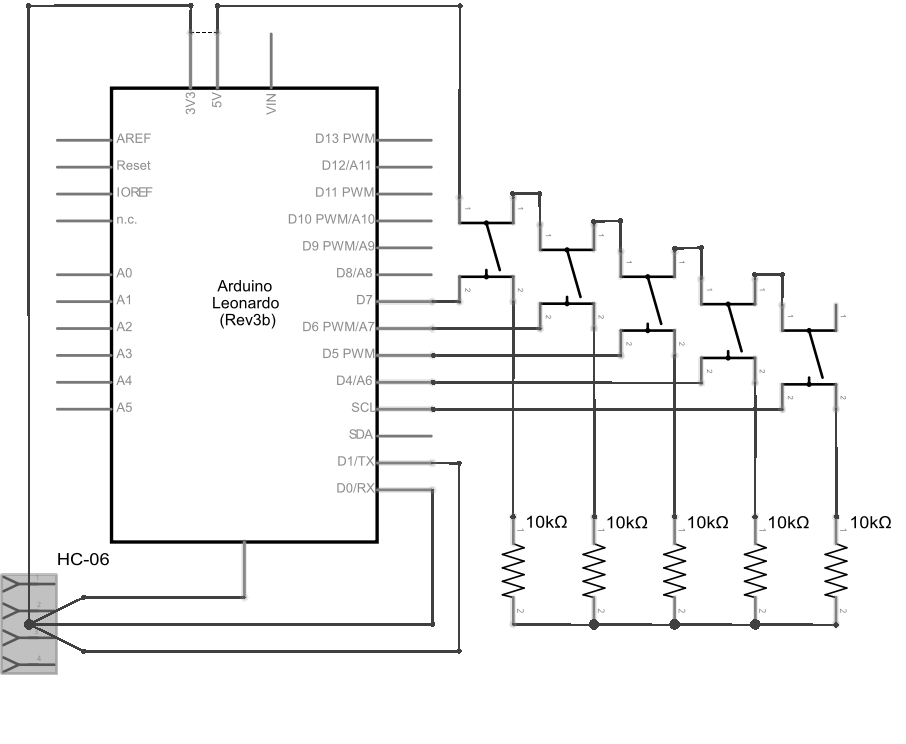
\includegraphics{mediaController_schem}}
				\caption{A circuit diagram of the proposed media-controller}
			\end{figure}
		
		\subsection{Mobile Application Design}
			The premise for the mobile application was simple, to allow a user to access the functions of the media-controller remotely, and as such the overall ascetic of the application was designed to be simplistic as well. The most challenging portion of the application's design stage was determining how the application would communicate with the micro-controller.
			
			\paragraph{Remote Serial Communication}
			Preliminary research indicated that two major technologies existed to communicate serial signals over-the-air namely; Bluetooth and Wi-Fi. A simplified breakdown of each standard is presented in Table~\ref{btWiFiComparison}.
			
			\begin{table}[h]
				\centering
				\caption{A comparison of two wireless communication technologies}
				\label{btWiFiComparison}
				\begin{tabular}{|r|r|r|r|r|r|}
					\hline
					\multicolumn{1}{|l|}{Technology} & \multicolumn{1}{l|}{Range} & \multicolumn{1}{l|}{Frequency} & \multicolumn{1}{l|}{Data Rate} & \multicolumn{1}{l|}{Power Use} & \multicolumn{1}{l|}{Cost} \\ \hline
					Bluetooth 2.0                    & $\sim$100m                 & 2.4 GHz                        & 1-3 Mbit/s                     & Medium                         & Low                       \\
					Wi-Fi 802.11g                     & $\sim$100m                 & 2.4 GHz                        & 54 Mbit/s                      & High                           & Medium                    \\ \hline
				\end{tabular}
			\end{table}
			
			\noindent
			As can be seen from the table, both technologies offer similar benefits and either could be used in the final system. In the end it was decided tat Bluetooth would be they most suitable medium, due to its lower cost and previous/personal experience using the technology. To finalise this decision, a HC-06 Bluetooth module \cite{HC06DataSheet:online} was purchased to allow the media controller to transmit a Bluetooth signal.
			
			\paragraph{Bluetooth Communication}
			While Bluetooth is a relatively simple technology in terms of use, it still must be correctly configured to ensure expected functionality. A activity diagram of the Bluetooth connection process [Appendix~\ref{AppBtActivity}] was created to ensure that the application's communication procedure was well documented and implemented correctly.
			
			\paragraph{User Interface}
			As previously stated, the goal of the applications interface was to keep as simple as possible. Wire frames were produced to prototype potential layouts. In the end a simple panel of vertical buttons was chosen for its ease of use and minimalistic style.\\
			
			\noindent
			//put in some figures of wire frames

	\section{Implementation}
		\subsection{Media-controller Implementation}
			With the knowledge that HID usage commands would be the most feasible way to complete the project the creation of a bespoke, media usage table was begun. However, to complete the implementation further examples of usage tables were required.
			
			By examining Arduino's default mouse and keyboard HID library's \cite{ArduinoGit:online} and utilizing information from the USB Implementers Forum \cite{USBHID:online} it became clear how to implement a usage table as an Arduino library. With the usage table implemented, it still had to be filled with the relevant hexadecimal codes.
				
			\paragraph{Usage Codes}
			A three year-old personal blog post that had previously been dismissed for being too outdated was able to provided a sample Usage Table with a host of different media commands \cite{MediaBlog:online}. The post in question had been analysed as potential solution to the project during the initial research phase. However, due to the age of the post and the fact the code was designed to interact with an IDE fourteen iterations out of date (at time of writing), it was deemed unusable. Even a brief conversation on the official Arduino IRC channel with a lead developer determined that the libraries needed to get the blog code running again were no longer available in the Arduino IDE.
					
			While the majority of the hex codes presented in the blog's table were usable, a few were depreciated and no longer worked. The USB Implementers Forum once again provided the answer in the form of a PDF with all the current in use hex codes \cite{HIDUsagePage:online}.
			
			The usage codes used in the finished device are visible in Table~\ref{usageTable}, an example of how they appear in the source code is seen in [Appendix~\ref{mediacpp}]. 
			
			\begin{table}[]
				\centering
				\caption{A usage table of the HID commands utilized by the media-controller}
				\label{usageTable}
				\begin{tabular}{|r|r|r|}
					\hline
					\multicolumn{1}{|l|}{Usage ID} & \multicolumn{1}{l|}{Usage Name} & \multicolumn{1}{l|}{Usage Type} \\ \hline
					0xCD                           & Play/Pause                      & OSC                             \\
					0xB0                           & Play                            & OOC                             \\
					0xB1                           & Pause                           & OOC                             \\
					0xB3                           & Fast Forward                    & OOC                             \\
					0xB4                           & Rewind                          & OOC                             \\
					0xB5                           & Scan Next Track                 & OSC                             \\
					0xB6                           & Scan Previous Track             & OSC                             \\
					0xB7                           & Stop                            & OSC                             \\
					0xE2                           & Mute                            & OOC                             \\
					0xE9                           & Volume Increment                & RTC                             \\
					0xEA                           & Volume Decrement                & RTC                             \\ \hline
				\end{tabular}
			\end{table}
			
			\paragraph{Push Buttons}
			Once the media library was implemented they had to be made accessible to the user. This was done through the use of an open source Arduino button library called Bounce2 \cite{Bounce2Git:online}. The reason for using a external library was to ensure that any electrical "noise" or interference would not cause the micro-controller to register a single button press as multiple, calling a media function several times when a user only wanted to use it once.
			
			Once the buttons had been made foolproof, it was a simple matter of having each button call a command from the media library, see Listing~\ref{lst:mediaButton}, and the physical system implementation was complete. 
			
			\lstinputlisting[caption = An example of how the media-controler executes a media command., firstline = 67, firstnumber = 67, lastline = 69, label = lst:mediaButton]{../../ARDUINO/mediaController_debounce/mediaController_debounce.ino}
									
		\subsection{Mobile Application Implementation}
			As previously stated and can be seen from figures, the goal of the applications design was to be a simple as possible. For this reason implementation of the user interface took very little time. The majority of the effort was spent on configuring the Bluetooth communication, ensuring the application still functioned in the event of an unexpected disruption to the media-controller connection.\\
			
			\noindent
			//screen-shots from application go here
			
			\paragraph{User Interface}
			As can be seen, (reference), when the application is not connected to the media-controller the option available to the user is the connection button. This is done to prevent a user from attempting to use a function when the media-controller is inaccessible and causing confusion.\\
					
			Once the user is connected to the physical system they will be able to access several buttons, each corresponding to a button on the physical media-controller. A user will also be able to disconnect from the bonded device, returning them to the starting stage of the application.
			
			\paragraph{Bluetooth}
			As previously mentioned, the majority of the applications development time was spent on implementing the Bluetooth connection process. Sample code from Google \cite{GoogleBluetooth:online} was used to produce a basic Bluetooth connection class, with further error checking and handling added as the application was tested. The implemented Bluetooth tests can be seen in the included activity diagram [Appendix~\ref{AppBtActivity}].
			
			\paragraph{Signal Transmission}
			Having the application communicate a requested media function to the micro-controller was a simple affair. When a button on the applications user interface was click, a unique character was transmitted over the Bluetooth's output stream. Examples of the code used can be seen in Listings~\ref{lst:androidButton}~and~\ref{lst:bluetoothOut}
			
			\lstinputlisting[caption = A example of the Android's application button code., label = lst:androidButton, firstline = 31, firstnumber = 31, lastline = 37] {../../ANDROID/MediaController/app/src/main/java/uk/co/sam/mediacontroller/MainActivity.java}
			
			\lstinputlisting[caption = The method  called when transmitting a charcter to the media-controller., label = lst:bluetoothOut, firstline = 228, firstnumber = 228, lastline = 235] {../../ANDROID/MediaController/app/src/main/java/uk/co/sam/mediacontroller/BluetoothHandler.java}
			
			\paragraph{Signal Reception}
			On the device side of the spectrum, the code to receive a signal from the application was also simple to implement. The media-controller is constantly listening on it's serial input stream and, upon reading a character it calls the relevant function. It should be noted that pressing one of the physical buttons on the controller has a higher precedence than the application and will be executed before the application's requested command. The code required for this functionality is seen in Listing~\ref{lst:leonardoBt}.
			
			\lstinputlisting[caption = The code utilized by the microcontroller to recive input from the Application., label = lst:leonardoBt, firstline = 85, firstnumber = 85, lastline = 109] {../../ARDUINO/mediaController_debounce/mediaController_debounce.ino}
			
			
	\section{Results}
		\subsection{Achievements}
			\lipsum[1]
			
		\subsection{Recommendations}
			\lipsum[1]
			
	\section{Future Work}
		\lipsum[1]
	
	\section{Conclusion}
		\lipsum[1]
		
	\section{Evaluation of Achievement}
		\lipsum[1]
		
	\begin{figure}[]
		\centering
		\label{fullSystem}
		{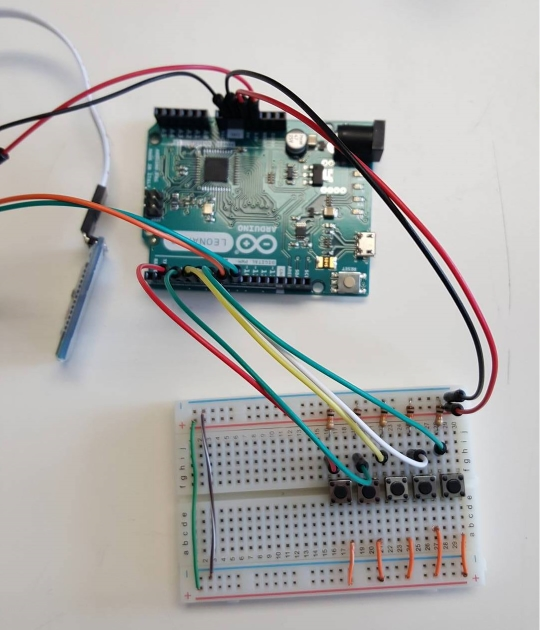
\includegraphics[scale = 0.5]{fullSystem}}
		\caption{The final media-controller complete with; micro-controller, Bluetooth module and push-buttons.}
	\end{figure}
	
%	\begin{figure}[]
%		\centering
%		\label{leonardo}
%		{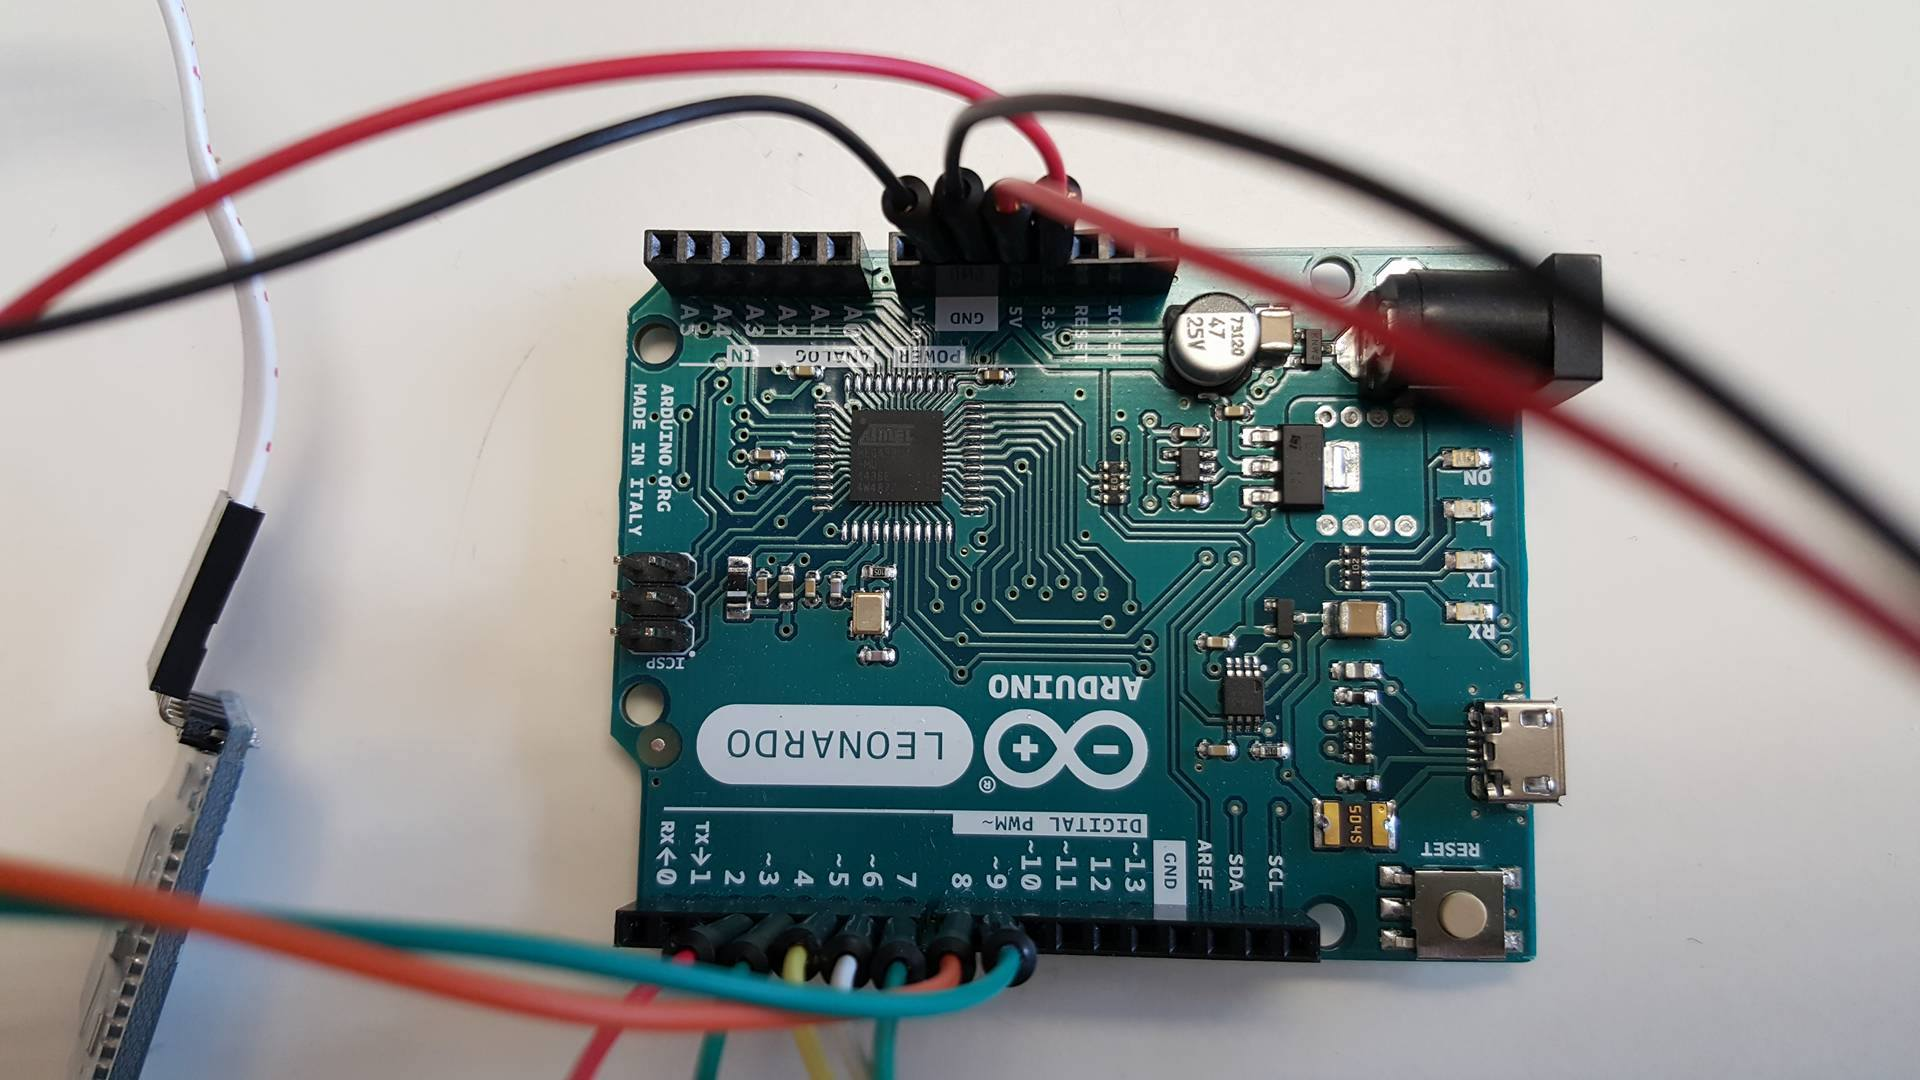
\includegraphics[scale = 0.15]{leonardo}}
%		\caption{//ToDo - Write a caption}
%	\end{figure}
	
%	\begin{figure}[]
%		\centering
%		\label{breadboard}
%		{\includegraphics[scale = 0.15]{breadboard}}
%		\caption{//ToDo - Write a caption}
%	\end{figure}
			
	\newpage	
		
	\addcontentsline{toc}{section}{References}
			
	\bibliographystyle{ieeetran}
	
	\bibliography{final}

	\newpage

	\begin{appendices}

		\section{Arduino Media-Controller Source Code}
			\lstinputlisting[title = mediaController\_debounce.ino, nolol]{../../ARDUINO/mediaController_debounce/mediaController_debounce.ino}
			
			\newpage
			
		\section{Arduino Media Key Library Source Code} \label{mediacpp}
			\lstinputlisting[title = Media.h, nolol]{../../ARDUINO/Media/Media.h}
			\newpage
			\lstinputlisting[title = Media.cpp, nolol]{../../ARDUINO/Media/Media.cpp}
			
			\newpage
			
		\section{Android Application Source code}
			\lstinputlisting[title = MainActivity.java, nolol]{../../ANDROID/MediaController/app/src/main/java/uk/co/sam/mediacontroller/MainActivity.java}
			
			\newpage
			
			\lstinputlisting[title = BluetoothHandler.java, nolol]{../../ANDROID/MediaController/app/src/main/java/uk/co/sam/mediacontroller/BluetoothHandler.java}
			
			
		\section{Bluetooth Connection Activity Diagram}
			\begin{figure}[H]
				\centering
				\label{AppBtActivity}
				\includegraphics*[scale = 0.75]{applicationConnectionActivity}
			\end{figure}
			
		\section{Arduino Leonardo Data Sheet}
		\begin{figure}[H]
			\centering
			\label{LeoDatasheet}
			\includegraphics*[scale = 0.75,angle=90]{ArduinoLeonardoDataSheet}
		\end{figure}
					
		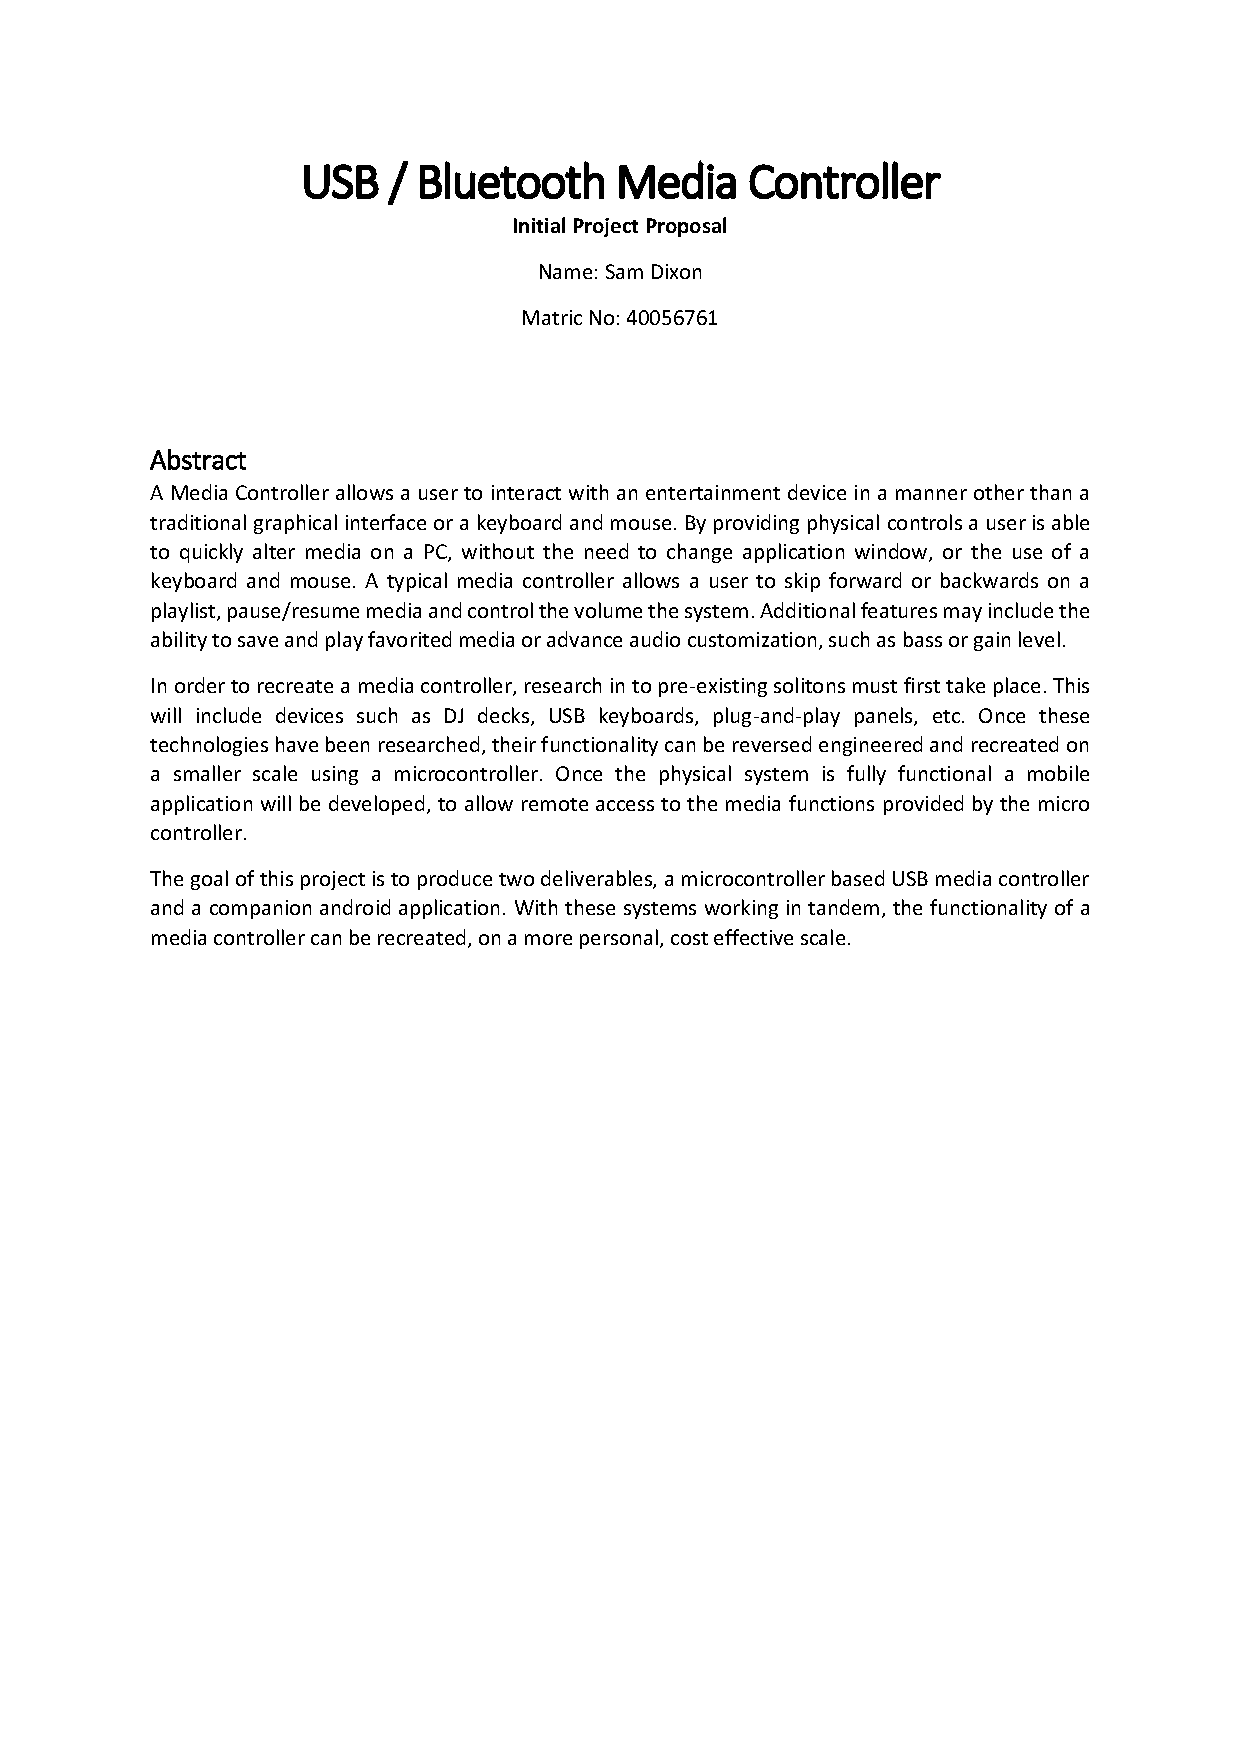
\includepdf[scale = 0.8, pages=1,pagecommand=\section{Initial Project Proposal}\label{IPP}]{../IPP/SET09118_IPP.pdf}
		\includepdf[scale = 0.8, pages=2-,pagecommand={}]{../IPP/SET09118_IPP.pdf}
		\newpage
	
		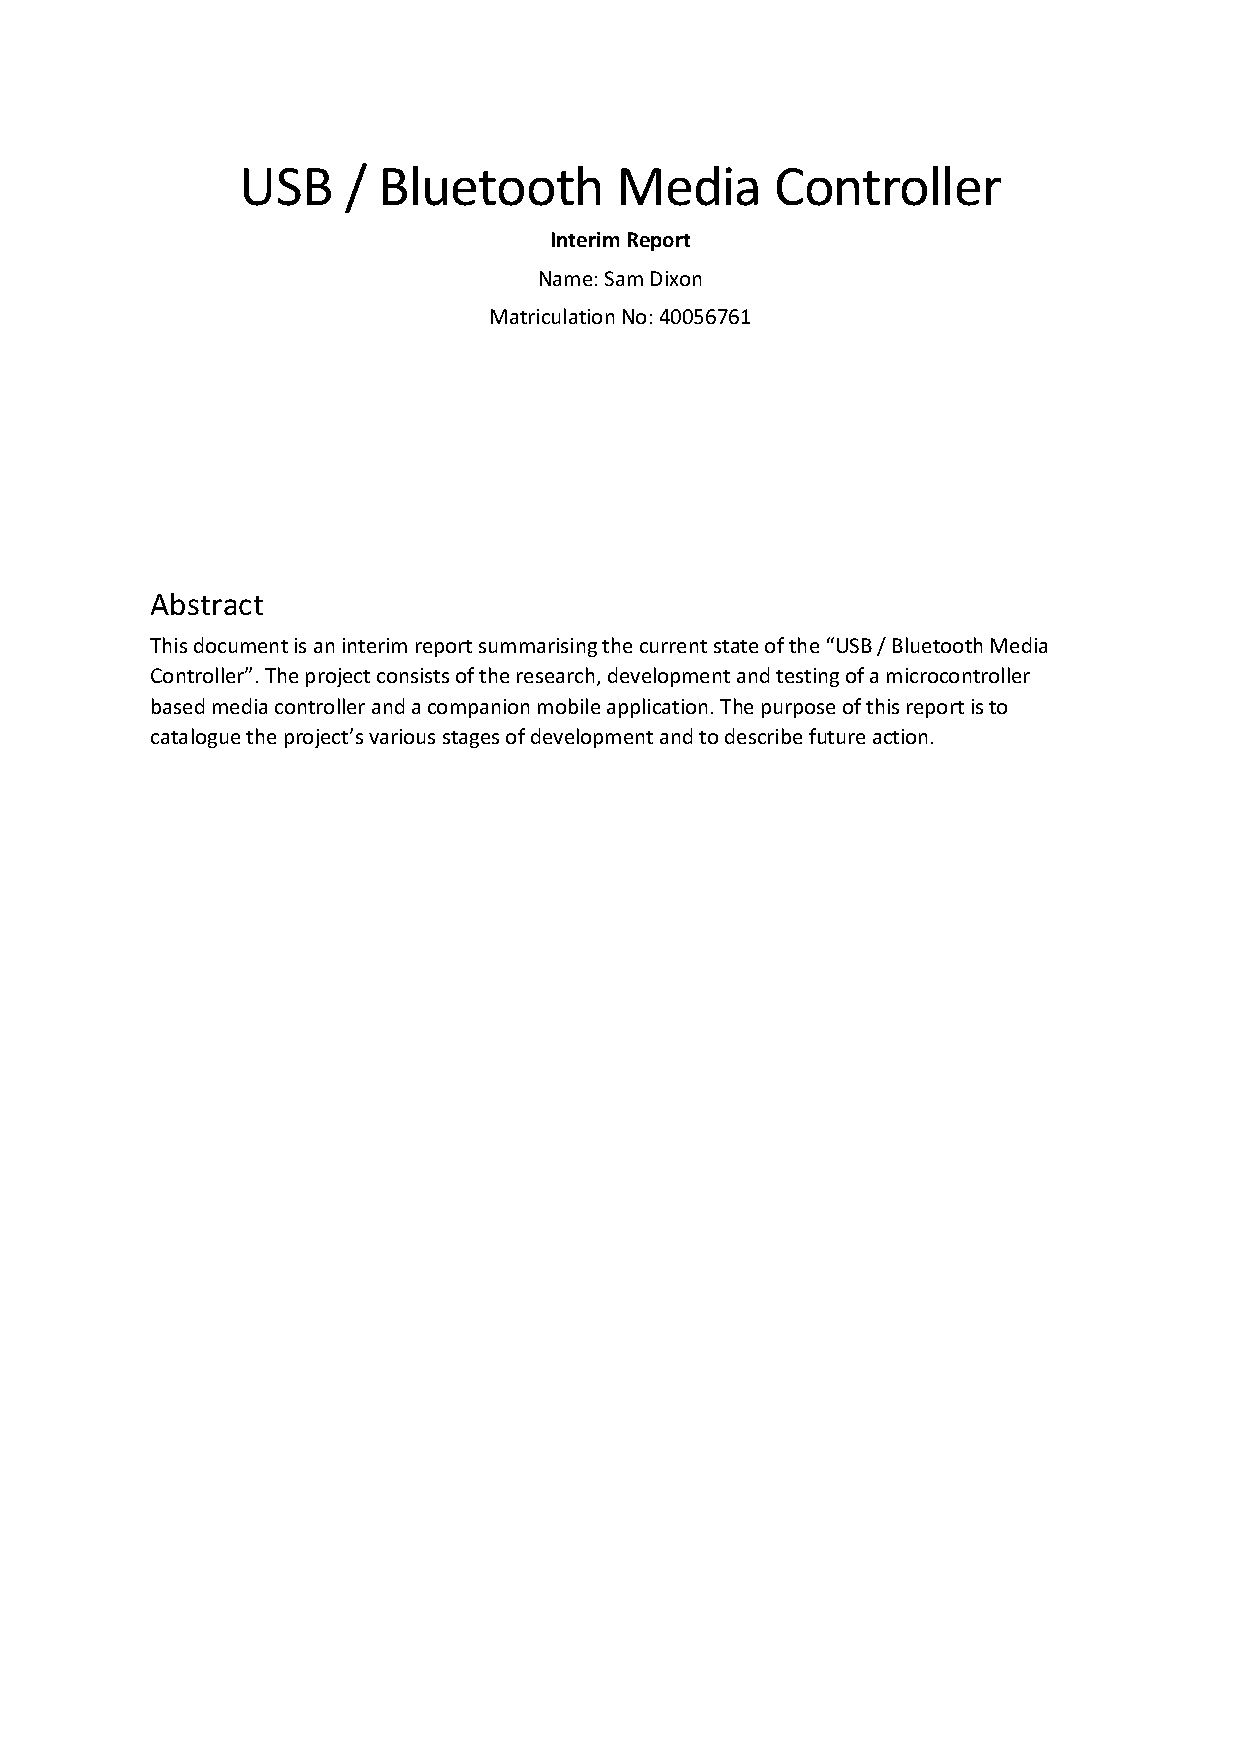
\includepdf[scale = 0.8, pages=1,pagecommand=\section{Interim Report}\label{Interim}]{../INTERIM/SET09118_INTERIM.pdf}
		\includepdf[scale = 0.8, pages=2-,pagecommand={}]{../INTERIM/SET09118_INTERIM.pdf}
		\newpage	
		 		
	\end{appendices}

\end{document}